%% ----------------------------------------------------------------
%%? 1st Draft In Progress
%% ----------------------------------------------------------------
\chapter{Project Planning Retrospective (1500 words)}
%todo fix the intro section
This section will explore in detail the planning and development of the project itself, throughout the stages: research, designing, development, evaluation and the final write-up.

I will go over what were the significant issues with the approach I took. I will then talk about how I would this project were I to start it over again.%todo make this sound better

Since this project had a very limited timeframe, ensuring that progress remained on schedule was critical. %? do I need to talk about how keeping things on schedule was important here?

%% ----------------------------------------------------------------
\section{What Went Well}
%% ----------------------------------------------------------------
One of the major elements that significantly helped with planning the project and managing the complexity of the project was building a hierarchical mindmap in Miro (a highly flexible diagramming tool). The reason Miro's mindmap was useful was that it allowed for children nodes to be toggled, meaning that they were visually hidden, but still accessible.

This meant that I could decompose the project into its significant core parts. Each section could then be decomposed into its significant parts. This significantly reduced the mental load and allowed for me to better breakdown each aspect of the project as much as I needed to.
\begin{figure}
    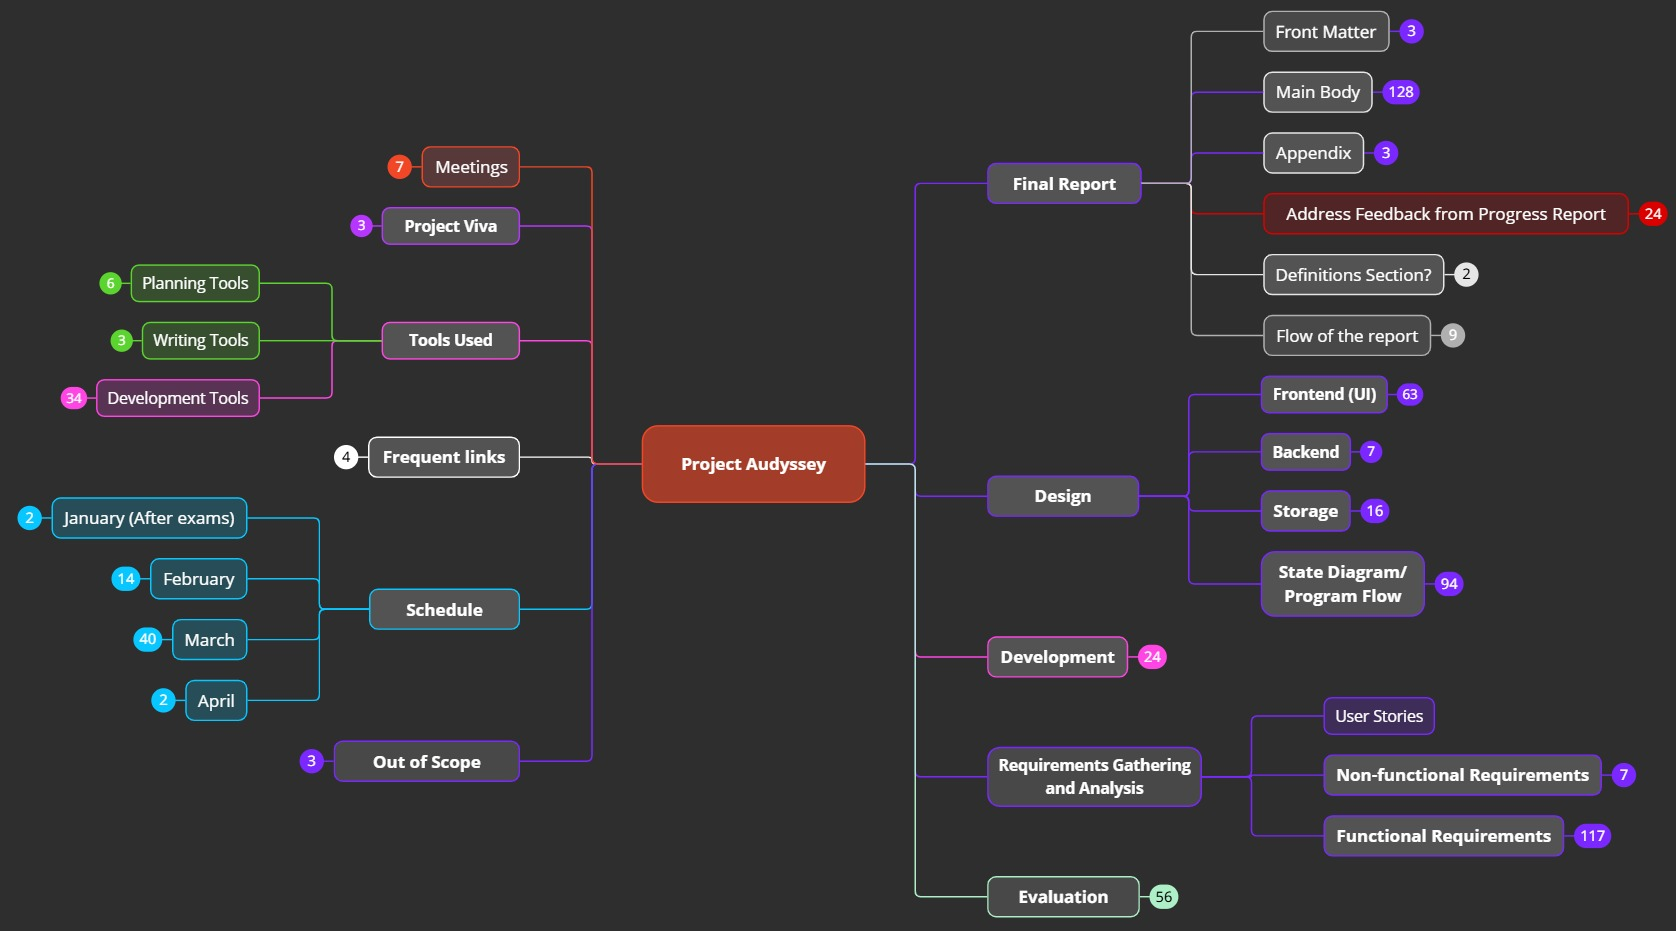
\includegraphics[angle=90, scale=0.434]{Miro_Mindmap_Depth_1,2}
    \caption{Miro Mindmap high level overview}
\end{figure}

%! Do I talk about how it also didn't work. Because I could hide stuff it was also a bit easier to forget about (about what???)

%% ----------------------------------------------------------------
\section{Limitations}
%% ----------------------------------------------------------------
There were some factors that limited this project:
[-] Unfinished Code limiting the ability to fully evaluate the concepts
    [-] spent too long on the Spotify and SoundCharts API stuff
    [-] lost 1-2 weeks due to LOpSoc and AdvCompArch
[-] Only got 6 people evaluated due to time constraints, still was very informative but more would've been better
    [-] ideally 8-10 participants to really see the patterns
[-] final evaluation was quite a lengthy process, should've done a mini user survey before the progress report to both find requirements and get an initial understanding. Then it would've been easier to see how the application and new concepts would've affected the listeners
[-] should've done more research into what the attributes that Spotify was offering were earlier in the research stage (not in the development stage) as that would have led to figuring out Exportify as the better route over SoundCharts.
    - In my defence, Spotify has obscured that the attributes were from the Echo Nest in their developer API.
    - they also deprecated the API endpoint days before the progress report handin, a significant milestone in the project meaning that as soon as an alternative was found, I had to take what I could get

%% ----------------------------------------------------------------
\subsection{Spotify Deprecating Access of Echo Nest Attributes}
%% ----------------------------------------------------------------
[2014] Spotify buys EchoNest - now EchoNest's API is locked behind a Spotify Premium Account (this wasn't an issue due to already having a premium account, but this is a paywall), however this was also a sort of blessing in disguise as it would've meant that I only need to work with one API.
    
[27 Nov 2024] Spotify announces they are deprecating several endpoints for applications made after the 27th November - these endpoints included both \lstinline|Get Track's Audio Features| and \lstinline|Get Track's Audio Analysis| which were key for the project

These audio features (or attributes) were necessary as they would provide the numerical basis for mapping the songs and helping control the audio journeys.

o ensure that this didn't derail the project, after much searching an alternative was found, namely the SoundCharts API. This API had an endpoint, that given a track's Spotify ID, would provide the attribute data that Spotify had deprecated access to.

However, this data was less accurate (only to 2 decimal places) and was also behind a paywall. For one month, the cost of access for 500,000 API calls at a 30\% academic discount amounted to 125 USD. This was within the budget of the project. Initially, the plan was to purchase one month once development had finished. As such the API access would be used only when it was fully needed.

[Late March 2025] Due to significant issues with purchasing the API access using the University's system, another alternative method to gaining the attributes had to be found. This solution was found in Exportify, a web tool built by Pavel Komarov. This tool accesses the Spotify API, including the newly deprecated endpoints, to allow for exporting a spotify user's library to a \lstinline|.csv| file.

This tool was made before the deprecation announcement and is free to use, making it a very suitable replacement. Futhermore, the attribute values are to the original precision as provided by Spotify. The tool also allowed for exporting of individual playlists, making it easier for my software application to know how one's full collection was composed by the playlists and the catch-all liked songs.

Unfortunately, due to the sudden nature of the Spotify deprecation announcement, an alternative had to be chosen very quickly meaning that Exportify wasn't found until very, very late in development. This meant that the API setup portion of the project took longer than it theoretically could've, as the workflow using Exportify's \lstinline|.csv| files is much simpler (as shown in the figure NUMBER below). The ideal method would've been to continue searching for alternatives after finding SoundCharts allowing for Exportify to be found sooner and be integrated into the application state flow from the start, however due to the time constraint in needing to submit a project brief, this was not done.%\includegraphics[]{} %todo Show the setup flow with SoundCharts versus with Exportify

SoundCharts - (good but not as detailed info, plus didn't give confidence interval endpoint and also paywalled which was an unreasonable amount of faff) - wasted a lot of time trying to get a workflow that allowed for not having to send repeated requests for the same song

%%? ----------------------------------------------------------------
\subsection{Unfinished Code in the Development Stage}
%%? ----------------------------------------------------------------
I didn't realise quite how much work it would be to develop the whole project. As such when the project reached a critical decision point in the development I made the wrong decision. Whilst the static graphs were useful for the project as explained in the evaluation section, I should've prioritised the dynamic journeys. This decision point came at a time when only one of the static or dynamic graph features would have time to be done properly.

Another reason is that I let other \textbf{subjects and responsibilities slow down progress too much}. (LOpSoc and AdvCompArch I guess??)

Progress was also slowed down by having a more complex application flow due to initially requiring SoundCharts API. Integrating Exportify's \lstinline|.csv| files meant that the setup state was simpler and make it easier to combine playlists when using the graph views. Unfortunately, due to switching to Exportify too late, there was no time reap these rewards.

%% ----------------------------------------------------------------
\subsection{
    Losing sight of the Goal
    Only learning and understanding the true goal of the project near the end.
}% Lost sight of the goal at the core of this project, which was the dynamic graph
%todo go over this bit again + make sure to add sources and cite if needed (such as when mentioning from the evaluation)
%% ----------------------------------------------------------------

This project whilst in a limited timeframe, was still quite long, having transpired over the better part of 7 months. During this process the true goal/research questions were only fully understood quite late into the project sadly.

\subsubsection{Static Cartesian Graphs: A Red Herring}
The true/original niche/gap in the research was investigating better ways to create listening journeys, mainly using the graph visualisations as a foundation for controlling and viewing them. This is because, with the advent of the digital streaming era, there has not been any research (none that I could find at least) for creating better tools for users. As discussed in the Evaluation, there is an expressed desire for these tools.

However, during development, after the static graph views were created, I realised that these were only really specifically useful in a data analysis perspective (something that has already been researched extensively and is not the focus of this project). The evaluation also confirmed this, as the participants felt that the static/cartesian graphs were only useful as a one-off and not as a basis for reflecting their mental model of their music collection.

In hindsight, developing the staic graph views should've been allocated to be done after the dynamic views so that the listening journeys could be accomplished as fast as possible. Static cartesian graphs were intially planned first as I did not realise at the time that they were significantly less useful for interacting with listening journeys than the dynamic view.

One participant in the evaluatory study also mentioned that they liked there being an absolute order to their songs/collection that they could return to. This absolute order synergises better with the dynamic graph, as the static graph produced different distributions for each combination of attributes on the axes.
%This was Vedarth, was there anyone else?

To prevent the static graphs feature be the 'red herring' that they were, in taking away development focus from the actual significant features (the dynamic graph and listening journeys) then this feature should've been omitted from the project during the research stage.
For this delay to have not occurred, the ideal scenario would've been to do more research in how the EchoNest attributes have been used much earlier in the project, before the design and development stages. 
During the research stage, more energy was invested into where to source the song attributes, meaning extensive research into how they had been used was only investigated during the development stage.

%However, this feature is not entirely destructive to this project as it confirmed that the cartesian static graph method of representing song libraries is not useful.

%%* Basically this feature wasn't good, but the main issue is that I should have pivoted during development to the dynamic graph once I realised I wouldn't have time to do both.

%%* It also helps show that the more unstructured view of the library where there is less detail is better for the general public to use on a more daily basis as it requires less mental effort to understand more
Whereas the more detailed in-depth view of the library by looking at the distributions of specific metrics is more useful when the person allocates a specific time to go through it.
This is because the view requires more mental energy to understand and explore it, to reach a sufficient mental understanding of it.

\subsection{Scope Creep: Implementing Better Listening}
Initially, as detailed in the project brief, this project aimed to create better listening queues by allowing for combinations of fixed and unfixed queues and greater flexibility in changing the directoin of the song queue.

%% ----------------------------------------------------------------
\section{Initial vs Final vs Ideal Project Plan}%todo find better name
%%? how much explanation do I need, will Gantt charts be enough
%% ----------------------------------------------------------------
Below are three project plans:\begin{itemize}
    \item \textbf{Initial Plan} \(\to\) this is what was planned initially near the start of the project
    \item \textbf{Actual Progress} \(\to\) this is the actual progress of the project
    \item \textbf{Ideal Plan} \(\to\) upon retrospection, this is how the project should be approached if to be done again
\end{itemize}

%% ----------------------------------------------------------------
\subsection{Initial Plan}
%% ----------------------------------------------------------------

%% ----------------------------------------------------------------
\subsection{Actual Progress}
%% ----------------------------------------------------------------

%% ----------------------------------------------------------------
\subsection{Ideal Plan}
%% ----------------------------------------------------------------

Key Points:
- reduce the amount of features
    - should've only done the dynamic graph as other people have done the static cartesian graphs before
    - the evaluation itself took ages 
- either of the below:
    - do an initial survey of people before design and development -> get a better sense of requirements
    - had a review meeting with the review team on the application - was supposed to do this but hadn't finished enough code in time and they both left the country early
    - minor thing, but should've asked if the action of skipping was annoying/effort